In contrast to the decade old neural network architectures like MLPs or convolutions, the \emph{transformer} architecture was only just introduced in 2017 with the works of \emph{Attention Is All You Need} \cite{attentionIsAllYouNeed}.
There, the \emph{scaled dot product attention} was established as a highly performant operator for use in \emph{natural language processing} (primarily - but not limited to - \emph{translation}).
In combination with other neural network components, the attention module was combined into the transformer.
The original transformer was designed for language tasks and therefore had several design elements that were implemented specifically to compute in that domain.

In the followup paper \emph{An Image is Worth 16x16 Words} \cite{imageWorth16x16} the \emph{vision transformer} was introduced and has since been improved upon numerous times \cite{swinTransformerPaper}.
As the transformer used in the experiments of this thesis is only a special case for the later introduced \emph{metaformer}, the transformer architecture will not be explained separately. 
This section will instead only introduce the attention calculation and related concepts.

\FloatBarrier
\paragraph{Attention} describes an algorithm, that allows a neural network to \emph{attend} to every presented bit of information at once, each scaled by learnable factors that depend on the currently processed input.
Specifically, the \emph{scaled dot product attention} mechanism will be discussed.

The algorithm for \emph{one attention head} is shown in \autoref{fig:attention-visualization}.
During the experiments, the transformers will use \emph{multi head attention}. 
The algorithm is exactly the same, but the calculation is repeated for multiple \glqq heads\grqq{} that all calculate the results independently with their own set of weights. 
Because of that, different heads can attend to the information with different strategies.

The algorithm starts with step 1, presented in \autoref{eq:attention-step-1}.
The input $x$ is used to calculate the queries $Q$, the keys $K$ and the values $V$, by matrix multiplying with the respective learnable weights $W^q, W^k$ and $W^v$.

Step 2 (\autoref{eq:attention-step-2}) is calculating the matrix $QK^\mathrm{T}$, by evaluation the \glqq outer product\grqq{} between $Q$ and $K$ (outer product in regards to the number of patches $n$).
As for big problem sets, $n$ can get quite large ($e$ is a fixed hyperparameter), this step is quite likely to be comparably expensive, as it has a complexity of $\mathcal{O}(n^2)$.
Especially for images, as $n$ doesn't describe the side length of a picture, but $n \propto h \cdot w$.
$QK^\mathrm{T}$ is a very important matrix, because it is a measure for the \glqq overlap\grqq{} of every key with every query. 
This is the core concept of the attention mechanism. 
The elements in $QK^\mathrm{T}$ are dot products of queries $q \in Q$ and keys $k \in K$. If $q$ and $k$ are \emph{parallel} - or in other words if the query and key align - the resulting output is going to be large.
If they are \emph{orthogonal} - speaking this is not the key the query is asking for - the value is going to be close to zero.

The steps 3 and 4 (\autoref{eq:attention-step-3-4}) are \emph{scaling} the values and taking the \emph{softmax}. 
This is to get \emph{interaction probabilities} out of the previously calculated quantities.

The last step 5 is listed in \autoref{eq:attention-step-5}.
The answer of the attention process $A$ is calculated as a weighted (with the interaction matrix $QK^\mathrm{T}$) sum of the values $V$ for each of the $n$ patches separately. 
This means for each of the $n$ entries of $x$, a \emph{query} is produced that is checked against all the other $n$ \emph{keys}. 
The degree of similarity determining the proportion, the corresponding \emph{value} is going constitute to the answer.

\begin{figure}[htbp]
    \centering
    \makebox[\textwidth][c]{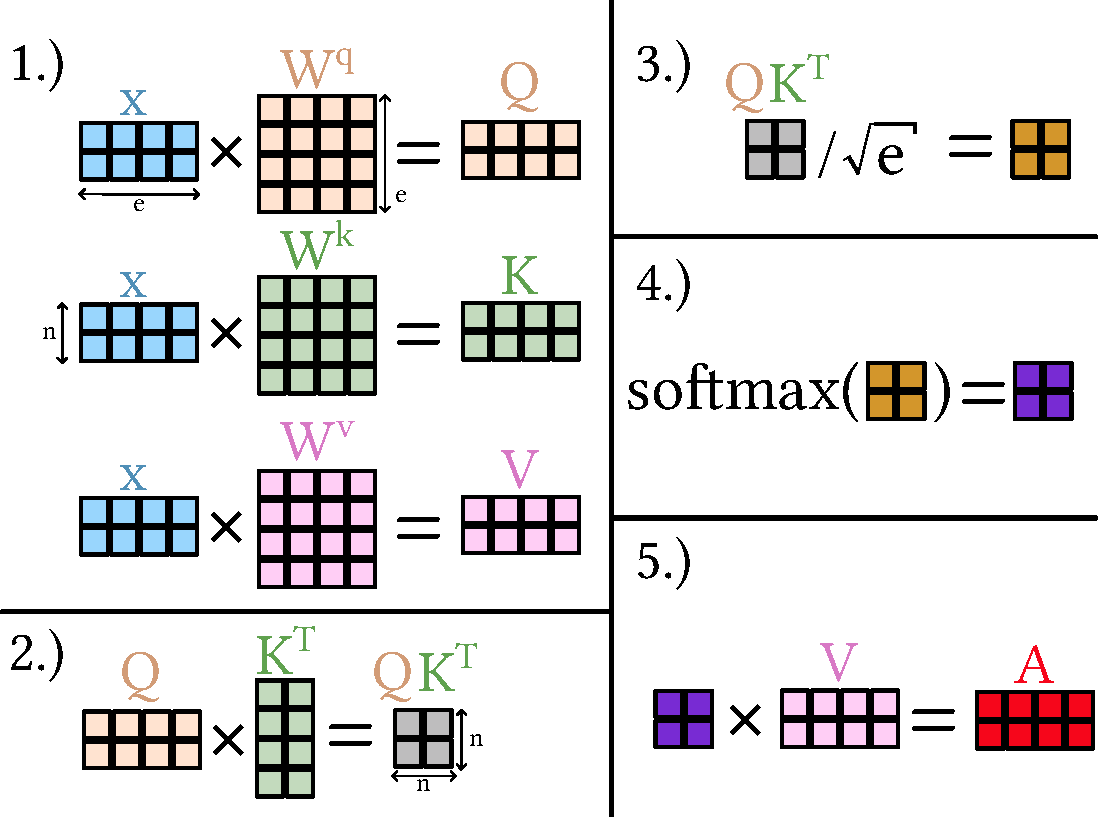
\includegraphics[width=0.8\textwidth]{./architectures/theory/attention/attention.pdf}}
    \caption{Schematic representation of the attention algorithm to picture the interacting dimensions.
            Only one attention head is pictured.
            In this example, the number of patches $n=2$ and the embed dimension $e=4$.
            Figure inspired by \cite{attentionVisualizationDimensionality}, but modified.
            }
    \label{fig:attention-visualization}
\end{figure}

\begin{equation}
    \label{eq:attention-step-1}
    Q = x \cdot W^q \qquad K = x \cdot W^k \qquad V = x \cdot W^v
\end{equation}
\begin{equation}
    \label{eq:attention-step-2}
    M = Q\cdot K^\mathrm{T}
\end{equation}
\begin{equation}
    \label{eq:attention-step-3-4}
    M' = \mathrm{softmax}\left(\frac{M}{\sqrt[]{e}}\right)
\end{equation}
\begin{equation}
    \label{eq:attention-step-5}
    A = M' \cdot V
\end{equation}

The implementation of the algorithm for multiple heads in parallel is appended in \autoref{appendix:attention}.

\FloatBarrier
\paragraph{Positional encoding} is an additional module, that can be used to boost the performance of a transformer.
The method works by (additively) enriching the embedded tokens with \glqq metadata\grqq{}, that gives the transformer vital information about the original location of the tokens.

During the attention computation, the model can take in information from any location at the same time, whilst there are no discernible differences between two patches of the same content but from different origins.
As it is clear, that the same word can have a different meaning, depending if it is located at the start or the end of a sentence, this is an obvious drawback of the attention module. 
For convolutions the direction and distance (and for pooling at least the distance) that a bit of information has traveled can be inferred, depending on the module's depth and size of the kernel. 
As this is impossible in the attention calculation, the encoding is used to provide this helpful information to the model.

The positional encoding is a unique vector that represents a position in the input sentence/image.
It can either be learned as part of the trainable parameters (implementation reference: \cite{dinoGithub}) or be predefined (fore example a \emph{sinusoidal encoding} - implementation reference: \cite{positionalEncodingGithub}).
The encoding either gets appended or added on top of the embedded token's value.

\begin{figure}[htbp]
    \centering
    \makebox[\textwidth][c]{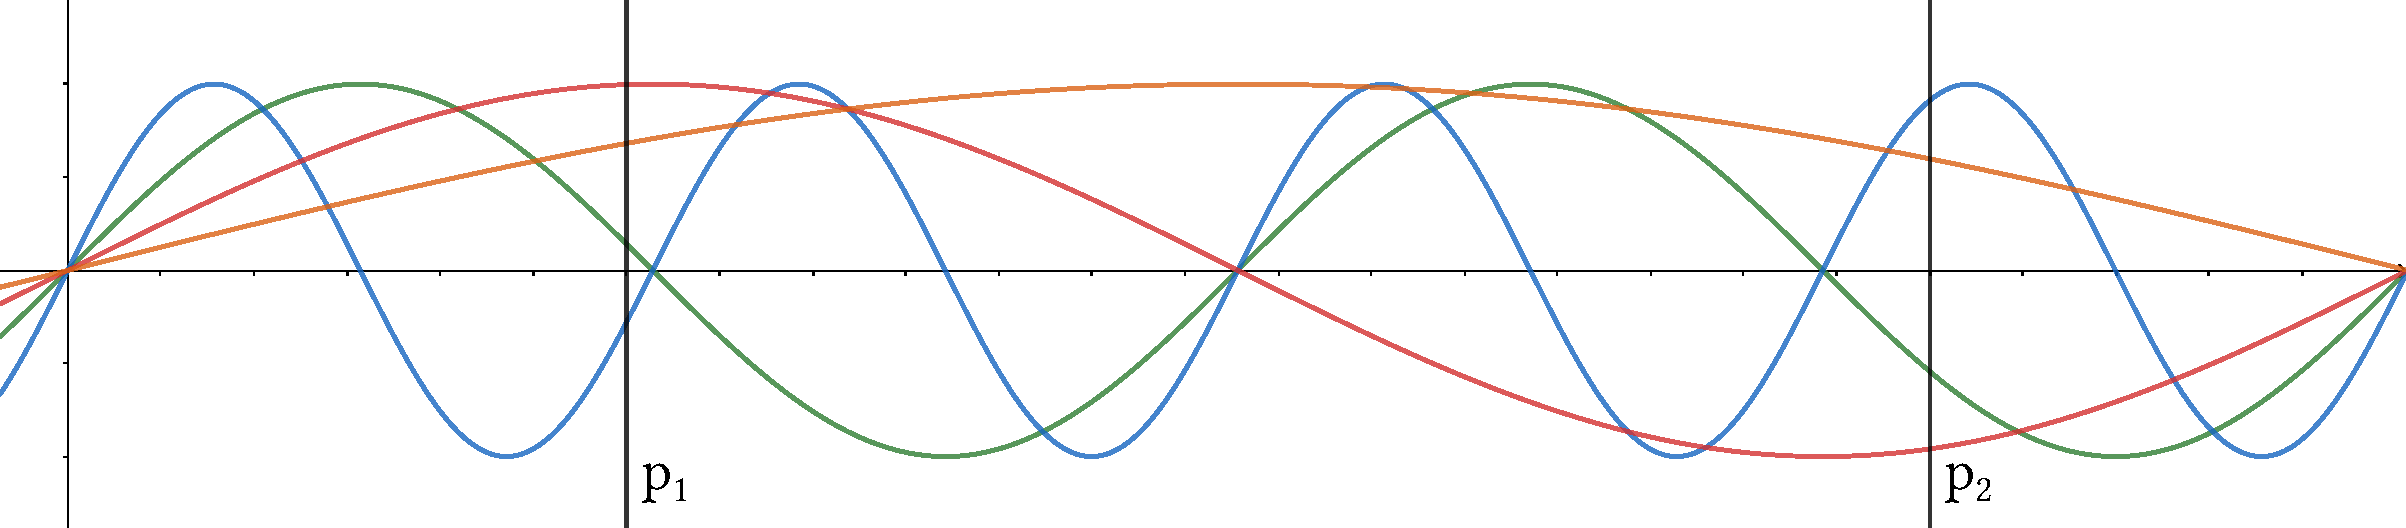
\includegraphics[width=0.9\textwidth]{./architectures/theory/attention/positional-encoding.pdf}}
    \vspace{0.1cm}
    \caption{Visualization of the sinusoidal positional encoding for an one-dimensional structure.
            The curves are sinusoidal waves with different frequencies. 
            The encodings can be sampled at arbitrary positions, and always give out a different encoding vector (if the frequencies are chosen accordingly).
            The distance of the sampled positions can be extracted from the encoded vectors.
    }
    \label{fig:positional-encoding}
\end{figure}

In \autoref{fig:positional-encoding}, a sinusoidal positional encoding is visualized. 
The corresponding encoding values are presented in \autoref{eq:positional-encoding}.

\begin{equation}
    \label{eq:positional-encoding}
    e(\mathrm{p}_1) = \left(\begin{matrix}
        \textcolor{textblue}{-0.279}\\
        \textcolor{textgreen}{\phantom{-}0.141}\\
        \textcolor{textred}{\phantom{-}0.997}\\
        \textcolor{textyellow}{\phantom{-}0.682}\\
    \end{matrix}\right)\qquad
    e(\mathrm{p}_2) = \left(\begin{matrix}
        \textcolor{textblue}{\phantom{-}0.913}\\
        \textcolor{textgreen}{-0.544}\\
        \textcolor{textred}{-0.959}\\
        \textcolor{textyellow}{\phantom{-}0.598}\\
    \end{matrix}\right)
\end{equation}